
% --------------- 12 POINT FONT -------------------------------
\documentclass[12pt]{article}
% --------------- 10 POINT FONT FOR CAPTIONS ------------------
\usepackage[font=footnotesize]{caption}
% --------------- NY TIMES FONT -------------------------------
\usepackage{times}
% --------------- 1 INCH MARGINS ------------------------------
\usepackage[margin=1in]{geometry}
% --------------- LINE SPACING --------------------------------
\usepackage{setspace}
\singlespacing
%\doublespacing
% --------------- SMALL SECTION TITLES ------------------------
\usepackage[tiny,compact]{titlesec}
% --------------- PACKAGES ------------------------------------
\usepackage{bookmark}
\usepackage{algorithm}
\usepackage{algpseudocode}
\usepackage{amsfonts}
\usepackage{amsmath}
\usepackage{amssymb}
\usepackage{amsthm}
\usepackage{bm}
\usepackage{color}
\usepackage{comment}
\usepackage{float}
\usepackage{graphicx}
%\usepackage[hidelinks]{hyperref}
\usepackage{makecell}
\usepackage[caption=false,font=footnotesize,subrefformat=parens,labelformat=parens]{subfig}
\usepackage{wrapfig}
\usepackage{url}
\usepackage[table]{xcolor}
\graphicspath{{images/}}
\begin{document}
% --------------- TITLE AND NAME ------------------------------
\begin{center}
\textbf{Summary}\\
\end{center}

\noindent
Bardia Mojra\\
\today\\
Seminar on Continual Learning\\
Robotic Vision Lab\\
% --------------- CONTENT -------------------------------------
\begin{center}
A Simple Approach to Continual Learning By\\
Transferring Skill Parameters\\
\end{center}
\begin{center}
  {\small K.R. Zentner, Ryan Julian, Ujjwal Puri, Yulun Zhang, and Gaurav S. Sukhatme}\\
\end{center}

Learning robotic manipulation tasks from vision is challenging and requires
massive amount of data and hundreds of hours of training. In recent years,
physics-based simulators and Deep Reinforcement Learning (DRL) algorithms have
been widely
used to allow learning agents to explore the solution space and construct rich
function approximators or policy functions. In such end-to-end approaches,
researchers train a Deep Neural Network (DNN) with both visual input and
motor control output data provided at the same time but rather in short and
similar episodes. Nonetheless, the main issue with this approach is the fact
that it is still too computationally expensive to learn new skills from scratch or
to even retrain after transfer learning.\\

\noindent
The authors introduce a novel and more efficient method for
continual learning of manipulation tasks by transferring skill parameters. They
show that representing past experiences only in form of skill policies,
methodical pretraining, and appropriately choosing when to
transfer those skill policies is a simple yet effective recipe for building a
continual learner in the context of robotic manipulation. New skill policies are
learned based on \textit{prior skills} or \textit{skill libraries} to enable
efficient acquisition and transfer of dynamic control policies. Similar to
\cite{hausman2018learning} and \cite{julian2018scaling}, they train reuseable
skill libraries in simulation to develop composable skill policies in form
of latent space parameter.\\


\noindent
\textbf{Setting}
They define continual learning problem as iterated transfer learning for
multi-task reinforcement learning (MTRL) on a possibly-unbounded discrete space
of tasks \(\mathcal{T}\).
S a single continuous state space shared among all tasks T.
A a single continuous action space shared among all tasks T.
The MTRL problem is defined by \((\mathcal{T},~S,~A)\) and each task
\(\tau \in \mathcal{T}\) is an infinite-horizon Markov decision process (MDP)
defined as
\begin{equation}
\tau = \left(S, A, p_{\tau} (s,a,s'), r_{\tau} (s,a,s') \right).
\end{equation}
\noindent
Tasks are differentiated only by their reward functions \(r_{\tau}\) and
state transition dynamics \(p_{\tau}\). Thus, for simplicity they define
\begin{equation}
\tau = \left( r_{\tau}, p_{\tau}\right).
\end{equation}
\noindent
Importantly, the authors did not presume the robot has access to all tasks in
T at once or even a representative sample. The robot can only access one task at
a time. The time between task transitions is referred to as an 'epoch' with
each having a unique index. Tasks may reapear and when solving a "target task,"
the robot can only skill policies acquired while solving prior tasks M (the
"skill library"). Thus, they redefine the MTRL problem as
\begin{equation}
\tau = \left(S, A, M_{i}, p_{\tau_{i}} (s,a,s'), r_{\tau_{i}} (s,a,s') \right),
\end{equation}
\noindent
where \(M_i\) represents the set is manipulation skills the robot is initialized
with and \(i\) is the epoch number.
They primarily use PPO \cite{schulman2017proximal} for the RL algorithm F that
effectively samples the distribution of value function before training.\\

\noindent
\textbf{Simple Continual Learning with Skill Transfer}\\
\begin{figure}[h]
  \centering
  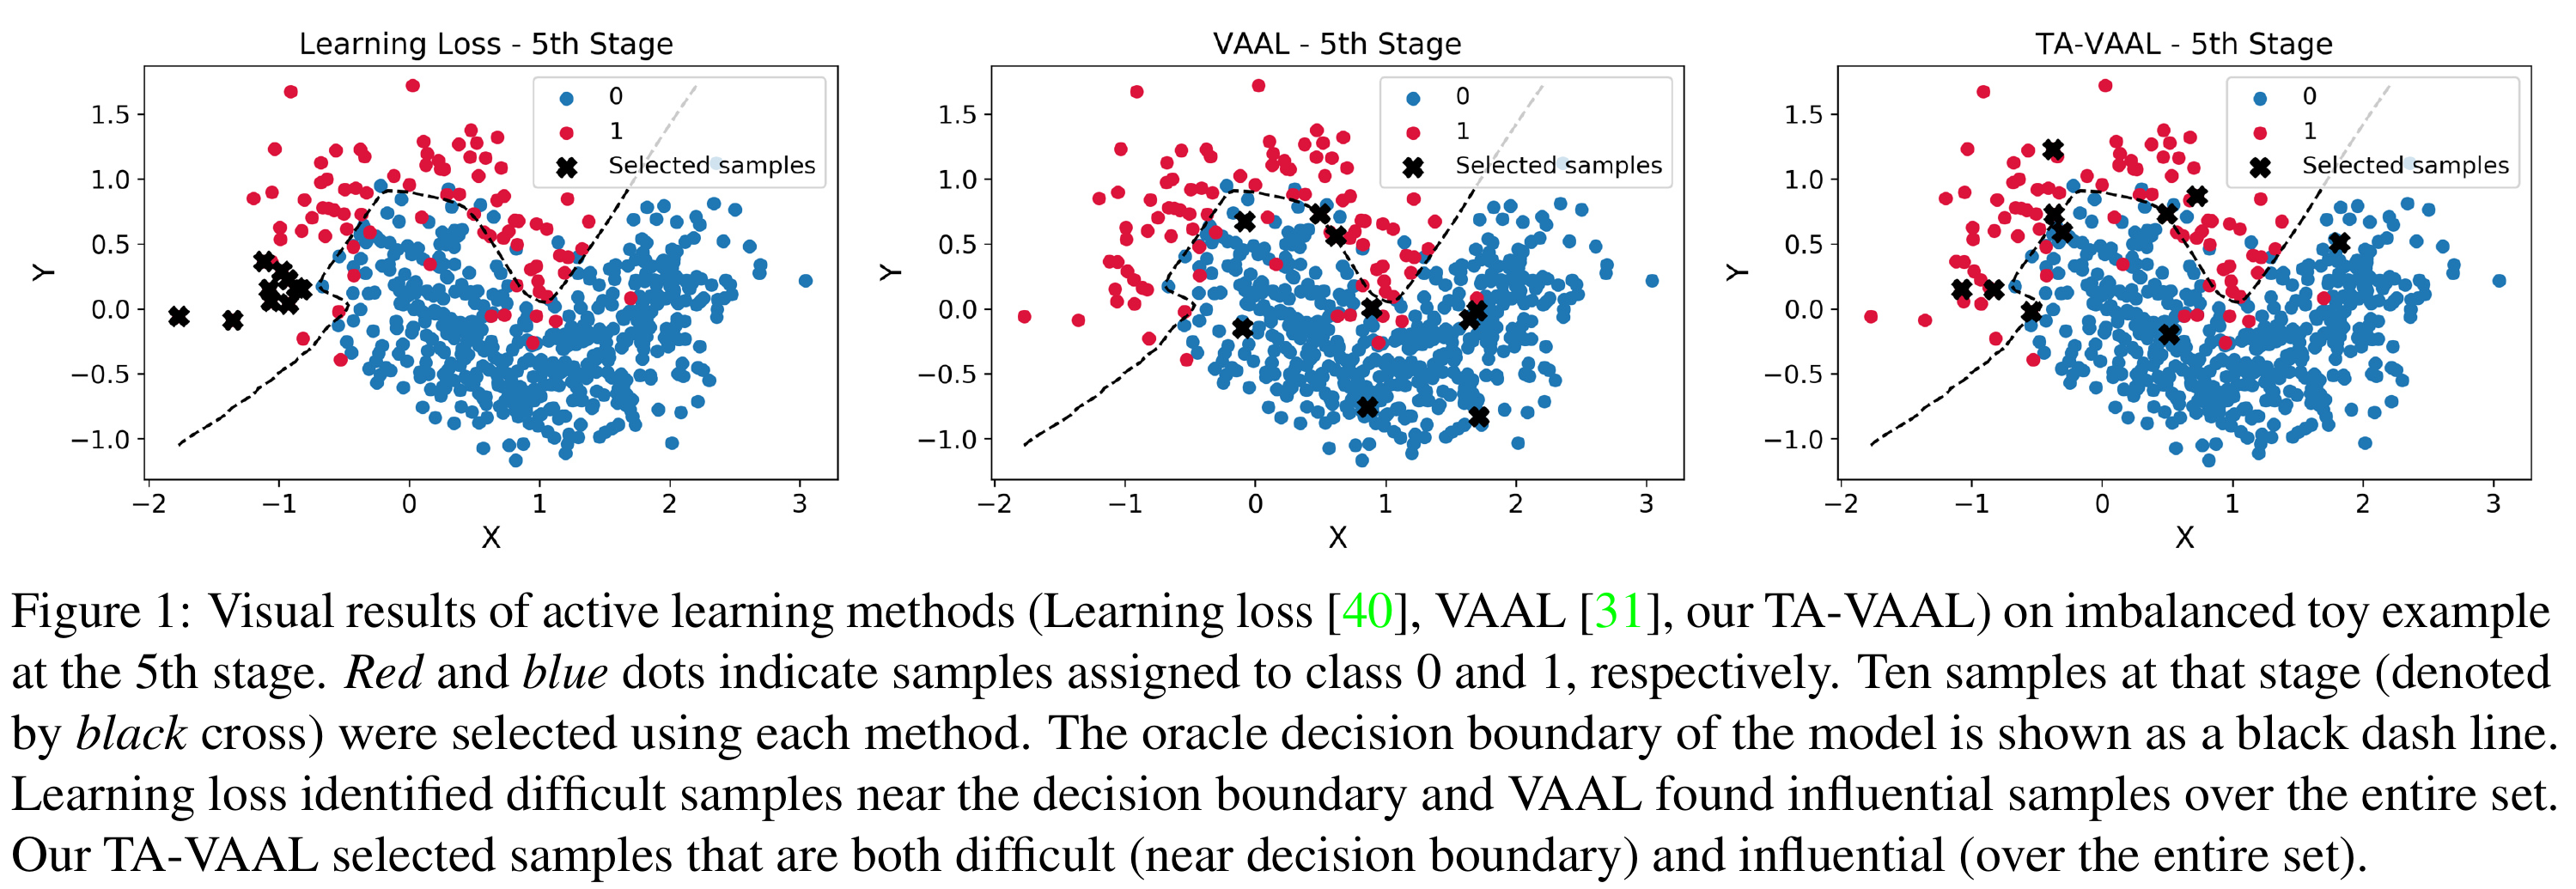
\includegraphics[width=1\textwidth]{/fig01.png}
  \caption{Algorithm 1}
\end{figure}

\noindent
\textbf{"Warm-Up" Procedure for Value Function Transfer} In order to tune a
skill on a task, they need a value function that estimates expected the reward
of that skill policy on the task \(\tau\). They used a initial gradient batch
sampling for estimating value function distribution similar to PPO. This allows
them to tune the value function of any skill on the new task and was necessary
to perform transfer effectively with PPO.\\

\noindent
\textbf{Rejecting Bad} Since new skills are build upon prior skills in a
hierarchial manner it is import to train and retain good transferred skills.
The authors built-in a mechanism where the learning agent can ternimate a
bad transfer at any time. It is characterized by a transferred policy \(\pi_{base}\)
that "falls too far behind" the from-scratch policy.\\

\noindent
\textbf{Skill-Skill Transfer Cost}
In order to transfer skills more efficiently, they tansformed the continual
learners training sequence form \textit{Random Skill Tranfer} to \textit{Skill
Curriculum}. Furthermore, they developed a method for measuring skill-skill
transfer cost by counting the number of samples needed to acquire a target Skill,
starting from a given base skill.\\

\newpage

\begin{figure}[h]
  \centering
  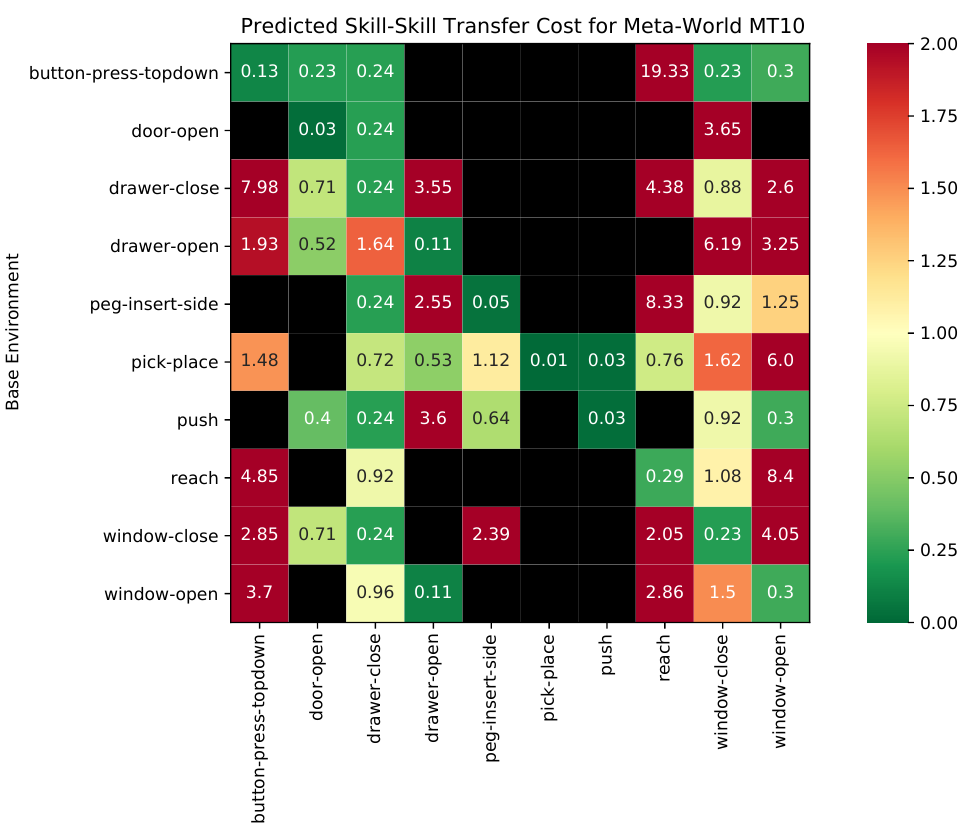
\includegraphics[width=.6\textwidth]{/fig03.png}
  \caption{Predicted Skill-Skill Transfer Cost}
\end{figure}

\noindent
\textbf{Predicted Skill-Skill Transfer Cost}
They define   as the ratio of time steps required to learn a task in MT10
\cite{meta-world} by skill transfer to learning the same task from scratch, using each
other possible skill policy as a base skill. Equation (4) and figure (2) show
skill transfer equation and scores, respectively.\\

\begin{equation}
A_{base \rightarrow target} = \frac{C_{base \rightarrow target}}{C_{scratch\rightarrow target}}
\end{equation}

\begin{figure}[h]
  \centering
  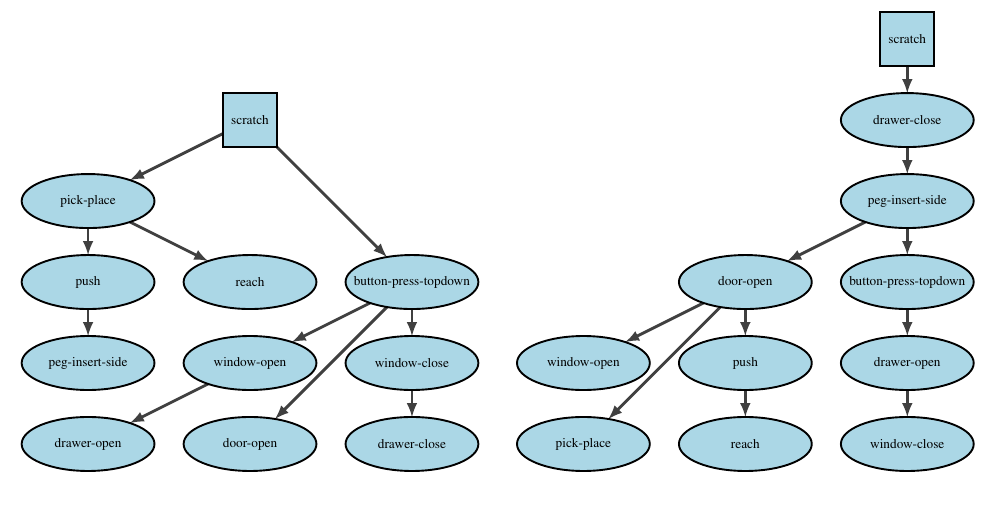
\includegraphics[width=.8\textwidth]{/fig04.png}
  \caption{Optimal and Pessimal Trees}
\end{figure}

\begin{figure}[h]
  \centering
  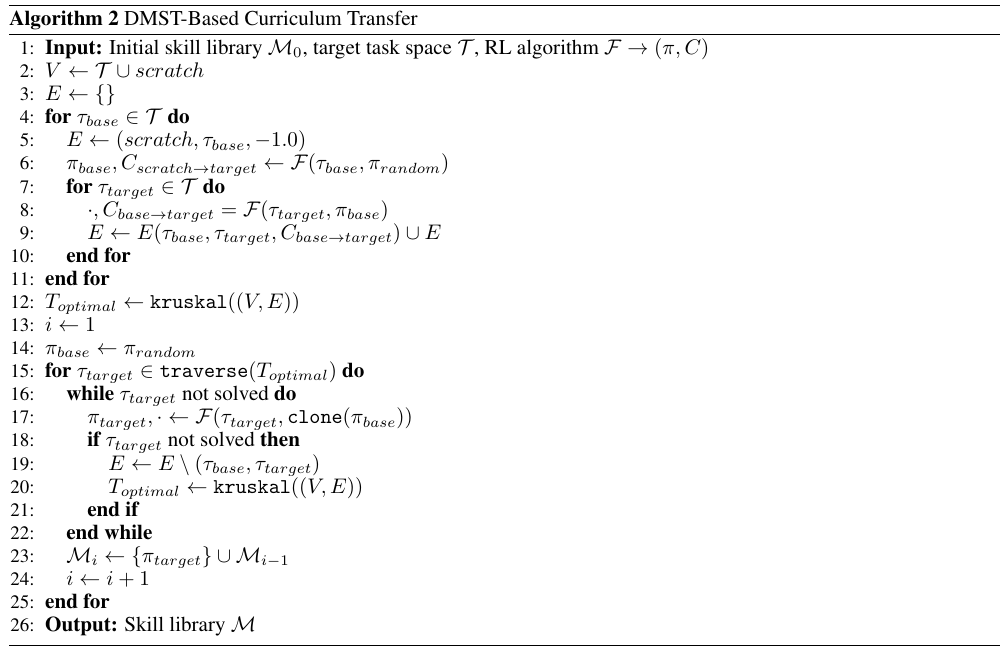
\includegraphics[width=1\textwidth]{/fig05.png}
  \caption{DMST-Based Curriculum Transfer Learning Algorithm}
\end{figure}

\noindent
\textbf{Curriculum Selection Algorithm}
They generate a skill-skill transfer cost for each task \(\tau \in \mathcal{T}\), which
form the weighted adjacency matrix of a densely-connected directed graph with
skill-skill transfer costs as the directed edge weights. With this problem
setting,
they solve for the Directed Minimum Spanning Tree (DMST) to obtain the optimal
path for sequentially transferring all tasks.
Thus, they create an optimal transfer learning curriculum for transferring and
retuning any skill. Figure (3) and (4) depict examples of optimal and pessimal trees
and DMST-based curriculum transfer learning algorithm, respectively.
Figure (5)
shows performance comparison between different skill curriculums for MT10.\\

\begin{figure}[h]
  \centering
  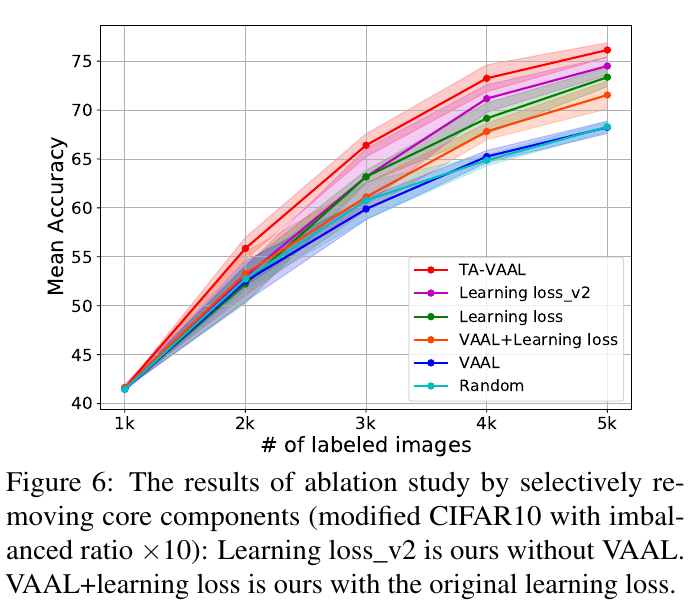
\includegraphics[width=1\textwidth]{/fig06.png}
  \caption{DMST-Based Curriculum Transfer Learning Algorithm}
\end{figure}




%Sets the bibliography style to UNSRT and import the
\newpage

\bibliography{ref}
\bibliographystyle{ieeetr}

\end{document}
